\documentclass[a4paper]{article}

\usepackage{color}
\usepackage{url}
\usepackage[T2A]{fontenc} 
\usepackage[utf8]{inputenc} 
\usepackage{graphicx}
\usepackage{parselines} 



\usepackage[english,serbian]{babel}


\usepackage[unicode]{hyperref}
\hypersetup{colorlinks,citecolor=green,filecolor=green,linkcolor=blue,urlcolor=blue}

\begin{document}
	
	\title{Entoni Džejms Bar\\ \small{Seminarksi rad u okviru kursa\\Tehničko i naučno pisanje\\Matematički fakultet}}
	
	\author{Divna Mićić\\ divna1999gmail.com \and
		Milica Golubović \\ milicagolubovic13@gmail.com \and
		Lucija Kecić \\ lkecic@gmail.com \and
		Nikola Borjan \\ nikola.borjan@yahoo.com} 
	
	\date{01.~novembar 2019.}
	
	\maketitle
	
	
	
	\abstract{\textbf{Entoni Džejms Bar} , poznatiji kao Toni Bar ili Džim Bar, rođen je 24. septembra 1940. godine. Američki je dizajner programskih jezika, inženjer softvera i izumitelj. Značajno je doprineo Sistemom statističke analize (SAS) (eng. Statistical Analysis System (SAS)) , automatizovao je optimizovanu potrošnju resursa drveta, kao i klasifikaciju medicinskih subjekata.
		
		\tableofcontents
		
		\newpage
		
		\section{Doprinos}
		
		\subsection{Sistem statističke analize}
		Sistem statističke analize (SAS), osmišljen od strane Bara 1966. godine, naišao je na široku primenu u nauci, upravi, industriji i akademskom razvitku. Septembra 1966., u gradu Atensu u Džordžiji, prezentovao je koncept njegove ideje članovima Odbora za Statistički Softver Univerzitetskih Statističara Južnih Eksperimentalnih Stanica (USJES).
		
		Bar je prethodno kreirao jezik za modelovanje analize slučaja, inspirisan notacijom statističara Morisa Kendala (eng. Maurice Kendall). Razvijao ga je u asemblerskom jeziku, na računaru IBM 1410, kao apsolvent državnog univerziteta Severne Karoline od 1962. do 1963. godine. Dr A. Grandedž, autor programa za analizu slučaja IBM 650, davao je savete o statističkim proračunima. Nakon toga je usledio višestruki regresijski program sa fleksibilnim ulaznim formatom i algebarskom transformacijom promenljivih, 1963. do 1964. godine. Na osnovu tih programa, zajedno sa svojim iskustvom sa strukturiranim datotekama podataka, kreirao je SAS, stavljajući statističke procedure u formatirani okvir datoteka.
		
		Bar je stekao iskustvo sa struktiranim datotekama podataka dok je radio na formatironom sistemu datoteka. Od 1966. do 1968. godine, Bar je razvio osnovnu struktru i jezik SAS-a.
		
		Bar je započeo saradnju sa drugima 1968. godine. Dizajnirao i implementirao programski jezik, upravljanje podacima, pisanje izvještaja i sistemska područja sistema koji se razvija. Entoni Dž. Bar, Džejms H. Gudnajt, Džon P. Sal i Džejn T. Helvig su 1976. godine osnovali Institut SAS, a Bar je imao najveći udeo (40\% ). Svoje akcije je prodao 1979.
		
		\subsection{Automatska klasifikacija medicinskih subjekata (AKMS)}
		AKMS je kompjuterski program koji određuje jedan primarni uzrok smrti na osnovu više uzroka smrti navedenih u umrlici. Bar je kreirao ovaj program za Nacionalni centar za zdravstvenu statistiku u periodu od 1967. do 1969. godine.
		
		AKMS zajedno sa drugim komponentama čini Sistem medicinskih podataka o smrtnosti. Ovaj sistem se koristi za određivanje uzroka smrti u svim umrlicama u SAD-u. AKMS je postao međunarodni standard za automatsku selekciju osnovnog uzroka smrti. Sadrži bitne podatke koji se koriste u proračunu statistike smrtnosti.
		
		\subsection{Automatska optimizacija potrošnje resursa drveta}
		Bar je 1971. i 1972. godine, u saradnji sa Sendijem Mulinom (eng. Sandy Mullin), dizajnirao, patentirao i sagradio prvu računarsku opremu za optimizaciju upotrebe drveta u industriji nameštaja. Uređaj je mogao da čita obeležene mane na daskama, izračunava potrebne rezove za optimalnu upotrebu dasaka i obeležava linije po kojima će se seći daske.
		
		Kompanija Bar-Mulin je osnovana 1973. godine, a njena tehnologija za optimizaciju upotrebe drveta se i dalje koristi u američkoj industriji drveta. 
		
		\subsection{Linker za IBM/360}
		Bar je 1968. kreirao prvi linker koji nije IBM-ov, za IBM/360. Nazvan je LDR, linker je sponzorisala Američka kompanija za obradu podataka iz Ralija, Severna Karolina. Barov linker je smanjio tipično vreme testiranja programa za dvadeset i pet posto. IBM nije ponudio ekvivalentni linker više od osamnaest meseci nakon što je Barov linker bio komercijalno dostupan.
		
		\subsection{IBM simulatori radnih stanica}
		Godine 1971, Bar je kreirao prvi HASP terminalni emulator koji nije IBM-ov. Na tržištu Univerzitetske računarske kompanije (eng. UCC), HASP emulator je dao značajno bolje performanse u odnosu na IBM 2780 emulator, koji je Bar 1969. godine razvio za istu kompaniju. Emulatori su razvijeni na PDP-8 miniračunaru i omogućili su COPE terminalima da komuniciraju sa računarima serije IBM/360 i IBM/370.
		
		Bar je 1971. godine takođe uveo HASP radnu stanicu za M \&  M kompjuterske industrije u Orindžu (Kalifornija). Implementiran na DGN minikompjuteru, program je postao daljinski serijski terminal Singer korporacije. I Singer i UCC su prodali svoj deo terminala Harris korporaciji, koja je nastavila da trguje proizvodima.
		
		\subsection{Formatirani sistem datoteka}
		Bar je u periodu od 1964. do 1966. godine radio za IBM, u okviru federalnih sistema u Pentagonu, u Vašingtonu. Tu je radio na NIPS formatiranom fajl sistemu (FFS). FFS, generalizovani sistem upravljanja bazama podataka za vraćanje i pisanje izveštaja, bio je jedan od prvih sistema za upravljanje podacima koji su iskoristili prednost definisane strukture datoteka za skladištenje podataka i efikastost pretraživanja.
		
		Određen da radi za Nacionalni vojni komandni centar, Bar je doradio i unapredio FFS, implementirajući tri od pet njegovih glavnih komponenti - preuzimanje, sortiranje i ažuriranje datoteka.
		
		Rad sa FFS-om upoznao je Bara sa potencijalom definisane strukture datoteka, koji je trebalo da postane osnovni koncept SAS-a.
		
		
		\newpage
		
		
		\section{Patenti}
		
		\begin{itemize}
			\item Metrike zadovoljstva i metode primene
			\item Uređaj i metoda za maksimalno iskorišćenje izduženih zaliha
			\item Uređaj za optimizaciju iskoristivosti komada dasaka i slično
			\item Uređaj i metoda za optimizaciju iskoristivosti komada dasaka i slično
		\end{itemize}
		
		\section{Publikacije}
		
		\begin{itemize}
			\item Manson,A.R.;Bar,E.Dž.;Gudnajt,J.H.(1975), „Optimalna strategija nulte memorije i tačne verovatnoće za Blekdžek sa 4 špila”, \textit{Američki statističar}, \textbf29(2): 84-88
			\item Bar,E.Dž.;Gudnajt,J.H.;Sal,J.R.;Helvig,J.H.(1977), \textit{SAS vodič za programere}, Rali, Severna Karolina: SAS institut, Inc.
			\item Bar,E.Dž.(1977), „Distribucija i održavanje SAS-a”, \textit{Računarske nauke i statistika: Deseti godišnji simpozijum o interfejsu, Specijalna publikacija NBS 503:}215-220
			\item Bar,E.Dž.;Gudnajt,J.H.;Sal,J.P.;Helvig,J.T.(1976), \textit{Korisnički vodič za SAS 76}, Rali, Severna Karolina: SAS institut, Inc.
			\item Bar, E.Dž.(1978): „Upravljanje podacima u SAS-u i interfejsima za druge sisteme”, \textit{Zbornik radova iz računarske nauke i statistike: Jedanaesti godišnji simpozijum o interfejsu, Institut za statistiku, Državni univerzitet Severna Karolina}: 261-264
		\end{itemize}
		
		
		\newpage
		
		\section{Obrazovanje}
		
		\begin{itemize}
			\item Osnovne akademske studije iz primenjene fizike, Državni univerzitet Severna Karolina, 1962.
			\item Master studije iz fizike, Državni univerzitet Severna Karolina, 1968.
			\begin{itemize}
				\item 1963. stipendista Nacionalne naučne fondacije da studira fizičku okeanografiju na Institutu za okeanografiju Vuds Houla
				\item 1963. stipendista Nacionalne naučne fondacije za Državni univerzitet Severne Karoline
				\item 1995. Istaknuti diplomirani student, Državni univerzitet Severna Karolina, Fakultet za fizičke i matematičke nauke
			\end{itemize}
		\end{itemize}
		
		\begin{parse lines}[\noindent]{#1\\}
				
		\end{parse lines}
		
		\begin{figure}[h!]
			\begin{center}
				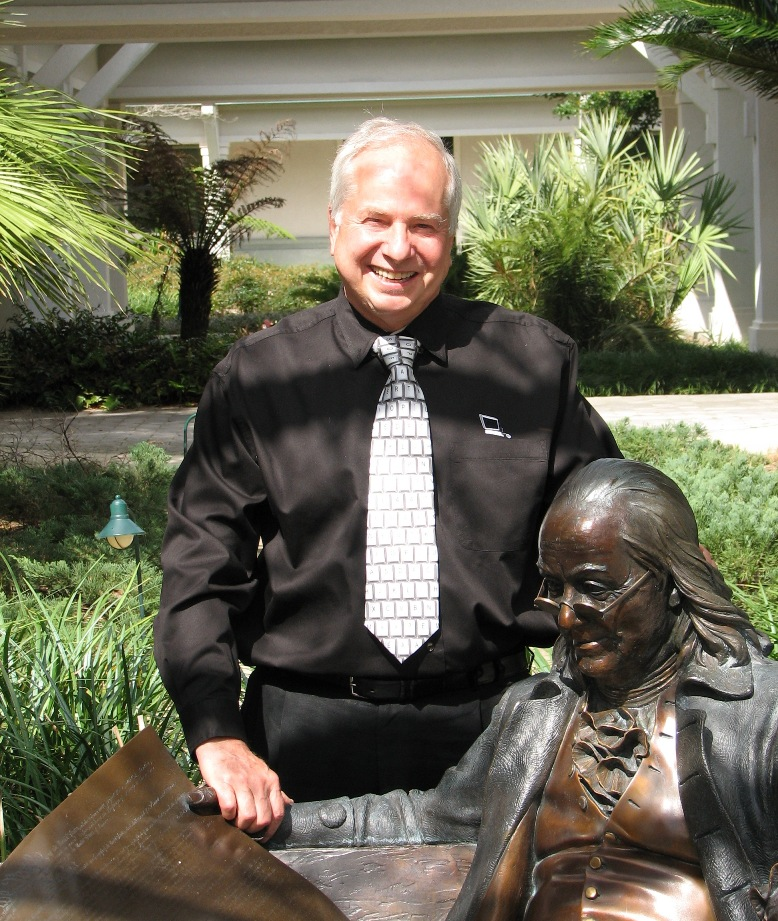
\includegraphics[scale=0.7]{TonyBarr.jpg}
			\end{center}
			\caption{Entoni Džejms Bar}
		\end{figure}
		

		\newpage
		
	


\section{Pregled tabelarno}
\begin{table}[h!]
	\begin{center}
		\begin{tabular}{|l|l|} \hline
			\multicolumn{2}{|c|}{\raisebox{0.6em} {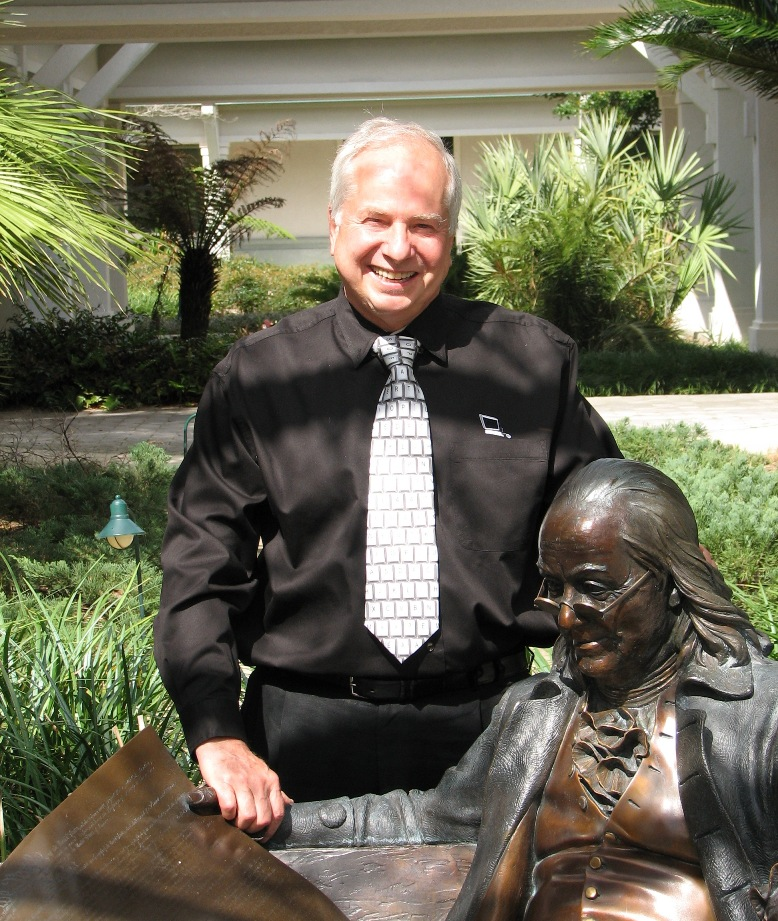
\includegraphics[scale=0.45]{TonyBarr.jpg}}}\\
			\multicolumn{2}{|c|}{Entoni Džejms Bar}\\ \hline
			\textbf{Datum rođenja} & 24. septembar 1940.\\ \hline
			\textbf{Druga imena} & Toni Bar, Džim Bar\\ \hline
			\textbf{Mesto rođenja} & Njujork, SAD\\ \hline
			\textbf{Obrazovanje} & Državni univerzitet, Severna Karolina
			\\ \hline
			\textbf {Zanimanje} & dizajner programskih jezika, softverski inženjer, pronalazač\\ \hline
		\end{tabular}
			\label{tab:tabela1}
		\end{center}
	\end{table}
	
	\addcontentsline{toc}{section}{Literatura}
	\appendix
	
	
	\bibliography{seminarski} 
	\bibliographystyle{plain}
	
	
	\appendix
	\renewcommand{\refname}{Reference}
	\begin{thebibliography}{brojReferenci}
		\bibitem{ime1} Ref 
		\bibitem{ime2} Ref
		
	\end{thebibliography}
\end{document}
